\begin{usecase}{Create Calendar}
    \ucbasicinfo{High}{Regular}
    \ucshortdescription{This UC allows the user to create a new calendar using iOS's native calendar system.}
    \uctrigger{This UC is triggered when the user clicks ``Create Calendar'' in the app.}
    \ucactors{User}{EventKit}
    \ucpreconditions{User must be logged in and have granted calendar access}
    \ucrelationships{N/A}{N/A}{N/A}
    \ucinputsoutputs{
        \begin{itemize}
            \item \textbf{Calendar name} (Source: User)
            \item \textbf{Calendar color} (Source: User)
        \end{itemize}
    }{
        \begin{itemize}
            \item \textbf{Calendar} (Destination: iOS Calendar System)
            \item \textbf{Calendar creation status} (Destination: App)
        \end{itemize}
    }
    \ucmainflow{
        \begin{enumerate}
            \item The user clicks the ``Create Calendar'' button in the app.
                  \ucinfo{The app asks the user to enter the calendar name and choose a calendar color.}
            \item The user submits the form for calendar information.
                  \ucinfo{The app uses EventKit to create a new calendar in iOS's calendar system.}
        \end{enumerate}
    }
    \ucalternateflows{
        \begin{itemize}
            \item If calendar creation fails, the user can retry through the app or any other app that uses EventKit.
        \end{itemize}
    }
    \ucexceptions{
        \begin{itemize}
            \item \textbf{Calendar access denied:} If the app doesn't have calendar access permission.
            \item \textbf{Calendar creation failure:} If iOS fails to create the calendar.
        \end{itemize}
    }
    \ucconclusion{The UC ends when the user has a new calendar created in iOS's calendar system.}
    \ucpostconditions{The new calendar appears in the user's iOS calendar system and is accessible through EventKit.}
\end{usecase}

\begin{figure}[!h]
    \centering
    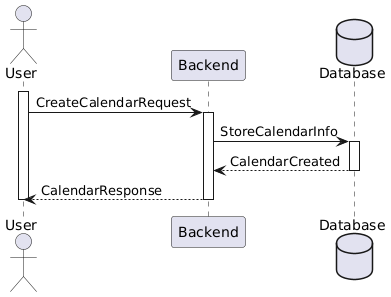
\includegraphics[width=0.5\textwidth]{images/docs/diagrams/sequence-diagrams/all-sequence-diagrams/Create Calendar.png}
    \caption{Create Calendar Sequence Diagram}
    \label{fig:seq/create-calendar}
\end{figure}

The ``Create Calendar Sequence Diagram'', shown in \textbf{Figure~\ref{fig:seq/create-calendar}}, illustrates how calendar creation is handled through iOS's native calendar system. When a user wants to create a new calendar, the app uses EventKit to interact with iOS's calendar system.

The process is straightforward:
\begin{enumerate}
    \item The app receives the user's calendar creation request with details like name and color
    \item EventKit is used to create the calendar in iOS's native calendar system
    \item The calendar becomes available to all apps with calendar access on the device
\end{enumerate}

This approach ensures that calendars are properly integrated with iOS's calendar infrastructure and can be accessed by other calendar apps on the device.